\documentclass[conference]{IEEEtran}
\IEEEoverridecommandlockouts

\usepackage[T1]{fontenc}
\usepackage[utf8]{inputenc}
\usepackage{cite}
\usepackage{amsmath,amssymb,amsfonts}
\usepackage{algorithmic}
\usepackage{graphicx}
\usepackage{textcomp}
\usepackage{xcolor}
\usepackage{booktabs}
\usepackage{tabularx}
\usepackage{enumitem}
\usepackage{url}
\usepackage{rotating}
\usepackage[hidelinks]{hyperref}
% Allow \path{} to break across lines at typical path separators so long
% file paths in tables do not overflow their column.
\Urlmuskip=0mu plus 1mu\relax
\makeatletter
\g@addto@macro{\UrlBreaks}{\do\/\do\-\do\_\do\.}
\makeatother
\hypersetup{
  pdfauthor={Aditya Sissodiya, Eric Chiquito, Johan Kristiansson, Ulf Bodin},
  pdftitle={Authority-Aligned Sequencing: Representing, Enforcing and Auditing Command Succession under Partition},
  pdfsubject={Working draft, reframed per AAS\_PLAN.md (not for submission)},
  pdfkeywords={command authority; succession of command; partition; leases and fencing; incident response; decision provenance},
  pdfproducer={},
  pdfcreator={}
}
% Suppress pdfTeX-generated CreationDate/ModDate and the random trailer ID so
% the build is reproducible: these fields otherwise vary per build and carry
% the build host's local timezone.
\pdfinfoomitdate=1
\pdftrailerid{}
\usepackage[nameinlink,noabbrev]{cleveref}
\usepackage{tikz}
\usetikzlibrary{positioning,arrows.meta,shapes.geometric,fit,backgrounds}
% Figure accents, shared with the matplotlib plots so one entity keeps one
% colour across the paper: accepted/normal path blue, fence/refusal orange.
\definecolor{accept}{HTML}{5B8DB8}
\definecolor{fence}{HTML}{C47B2C}

% Working-draft markers. \pending marks text that
% depends on the system model the supervisors have not yet agreed, or on
% results that have not yet been measured. Remove every one before submission.
\newcommand{\pending}[1]{\textcolor{fence}{[\textit{#1}]}}

\setlist[itemize]{leftmargin=*,topsep=2pt,itemsep=2pt}
\setlist[enumerate]{leftmargin=*,topsep=2pt,itemsep=2pt}

\newcommand{\systemname}{AAS}
\newcommand{\methodname}{authority-aligned sequencing}
% Auto-generated by scripts/plot_promotion_cdf.py.
\newcommand{\promotionN}{300}
\newcommand{\promotionNPerPhase}{100}
\newcommand{\promotionMedianCombined}{5.0\,ms}
\newcommand{\promotionPNinetyFiveCombined}{10.8\,ms}
\newcommand{\promotionMedianA}{6.3\,ms}
\newcommand{\promotionPNinetyFiveA}{14.0\,ms}
\newcommand{\promotionMedianB}{2.5\,ms}
\newcommand{\promotionPNinetyFiveB}{5.6\,ms}
\newcommand{\promotionMedianC}{5.7\,ms}
\newcommand{\promotionPNinetyFiveC}{10.7\,ms}

% Auto-derived from paper/data/eval_metrics.jsonl (command_throughput and
% command_throughput_endtoend, warm-up run excluded). events/s; units added in prose.
\newcommand{\TputDirectMedian}{356.3}
\newcommand{\TputDirectPNinetyFive}{491.7}
\newcommand{\TputEndToEndMedian}{159.4}
\newcommand{\TputEndToEndPNinetyFive}{163.9}

% Auto-generated by scripts/plot_netem_schedule.py.
% Do not edit; re-run the script after evaluation JSONL changes.
\newcommand{\scheduleRuns}{10}
\newcommand{\scheduleEvents}{540}
\newcommand{\schedulePeakBacklog}{13}
\newcommand{\scheduleDrainMedian}{0.93\,s}
\newcommand{\scheduleDrainMax}{1.12\,s}


\title{Authority-Aligned Sequencing: Representing, Enforcing and Auditing Command Succession under Partition}

\author{
\IEEEauthorblockN{Aditya Sissodiya, Eric Chiquito, Johan Kristiansson, and Ulf Bodin}
\IEEEauthorblockA{\textit{Cyber-Physical Systems research subject, Embedded Intelligent Systems LAB}\\
\textit{Department of Computer Science, Electrical and Space Engineering}\\
\textit{Luleå University of Technology}, SE-971 87 Luleå, Sweden\\
aditya.sissodiya@ltu.se, eric.chiquito@ltu.se, johan.kristiansson@ltu.se, ulf.bodin@ltu.se}
\thanks{The work presented in this paper was supported by Digitala Stambanan IndTech (Vinnova Reference Number: 2024-02510), and the Horizon Europe projects COP-PILOT under grant agreement 101189819 and RemaNet under grant agreement 101138627.}
}

\begin{document}

\maketitle

\noindent\pending{Working draft, not for submission; see AAS\_PLAN.md. The system model in \S~\ref{sec:system-model} is not yet agreed with the supervisors. Bracketed text in this colour marks open points or planned work, not results.}

\begin{abstract}
In rescue-service incident response, command belongs to a person: the incident commander, appointed by the organization. When that commander is cut off from the incident information system, the organization may hand command to a deputy or a superior, and the system must then decide which recorded decisions are authoritative. Clocks can order one person's decisions, but they cannot say whose authority was valid when two people each believed they were in command. We separate a person's right to command from a node's right to write. Authority comes from signed role grants and a succession rule that the organization fixes in advance; nodes exercise that authority but hold none of their own, and the network never decides who is in command. A decision is binding when it is admitted to the authoritative journal under a valid grant. Decisions made under a grant that had already been superseded are kept and labelled as residual, never merged or dropped. While the commander is cut off, a design can give at most two of three things: the commander keeps recording, command moves without the commander, and only one disconnected edge accepts decisions. We therefore treat succession as a choice of policy, compare six succession policies by what each one gives up, and place Authority-Aligned Sequencing (\systemname{}), our prototype, as one point in that space: immediate promotion through the regional core with a lease. We report what the prototype does and does not guarantee today, using a two-edge partition experiment, TLA+ model checking, and baselines against Raft and a last-writer-wins CRDT. \pending{A policy comparison across three partition cases is planned; no results yet.}

\end{abstract}

\begin{IEEEkeywords}
command authority, succession of command, network partition, leases and fencing, incident response, decision provenance
\end{IEEEkeywords}

\section{Introduction}
\label{sec:introduction}

Public-safety information systems must remain operational when commercial connectivity fails.
Rescue-service vehicles operate up to several hours away from regional dispatch centres. In that terrain, wireless connectivity alternates between full wide-area coverage, mesh-only operation, and total isolation~\cite{zimbelman2022mesh, wang2023overview}.
Disasters routinely degrade or destroy commercial telecom infrastructure precisely when
coordination demand is highest. In command-hierarchical environments the consequences of
information loss are wrong assignments, missed hazards, and conflicting orders.

The operational constraints are grounded in public Swedish rescue-service
guidance~\cite{rsg-rad201, rsg-kommunalplan}, which treats incident-planning information
as an ongoing, secrecy-restricted process rather than a static artifact; independent
studies of Swedish rescue-service information systems confirm these requirements and the
gaps in information flow~\cite{pilemalm2014enabling, westman2021mobilisation}.

Command at an incident belongs to a \emph{person}, the incident commander, appointed by
the organization. Every resource assignment, status transition, and command hazard
annotation---a \emph{decision}---carries that person's authority. The commander works
from a vehicle (Figure~\ref{fig:setting}), and that vehicle is often cut off from the
regional core. While it is cut off, the organization may decide that command passes to a
deputy or to a superior officer, usually agreed over voice radio. The information system
then holds decisions from two people, and it must say which of them are authoritative.

Ordering is not the hard part. One person cannot be in two vehicles at once, so a
per-person sequence number and GNSS time order that person's decisions, even across a
change of vehicle; epochs and leases are not needed for that case. The hard part is the
cut-over between two people's authority. Clocks give an order, not legitimacy: sorting by
time yields a tidy record of conflicting orders, such as ``engine~3 north'' from the cut-off
commander and ``engine~3 south'' from the deputy, without saying which one was valid.

\begin{figure}[t]
\centering
% The setting AAS operates in: incident site, regional core, intermittent links,
% who writes into the journal, and the command role that can move.
% Hand-drawn TikZ so it shares fonts and colours with Fig. 3: accepting path and
% messages blue (accept), refusal orange (fence). Link state is encoded by line
% style as well as by label: solid = local link, dashed = intermittent radio,
% dotted with a cross = link down.
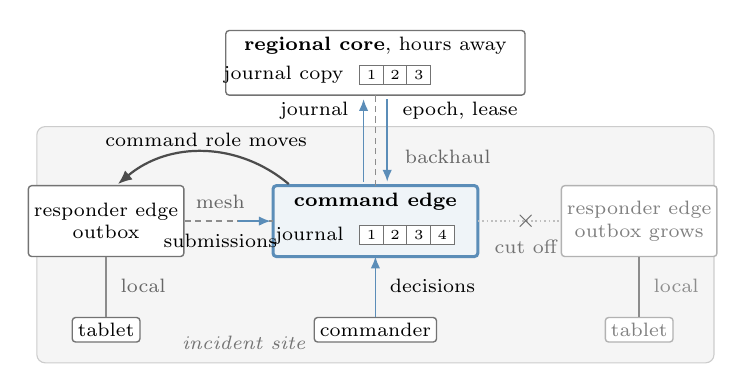
\begin{tikzpicture}[
  x=1cm, y=1cm,
  font=\scriptsize,
  box/.style={draw=black!55, rounded corners=1.2pt, fill=white, line width=0.5pt,
              align=center, inner sep=2pt},
  cmd/.style={draw=accept, rounded corners=1.2pt, fill=accept!10, line width=1.1pt},
  dim/.style={draw=black!30, rounded corners=1.2pt, fill=white, line width=0.5pt,
              align=center, inner sep=2pt, text=black!50},
  cell/.style={draw=black!55, fill=white, minimum width=0.3cm, minimum height=0.24cm,
               inner sep=0pt, font=\tiny},
  msg/.style={-{Latex[length=1.5mm,width=1.2mm]}, draw=accept, line width=0.6pt},
  local/.style={draw=black!45, line width=0.5pt},
  radio/.style={draw=black!45, line width=0.6pt, dash pattern=on 2.2pt off 1.6pt},
  down/.style={draw=black!25, line width=0.6pt, densely dotted},
  move/.style={-{Latex[length=1.8mm,width=1.5mm]}, draw=black!70, line width=0.8pt},
]
% Incident site: everything a rescue operation brings to the scene.
\draw[rounded corners=3pt, fill=black!4, draw=black!20] (0,0) rectangle (8.6,3.0);
\node[anchor=south west, font=\scriptsize\itshape, text=black!55] at (1.72,0.05) {incident site};

% Regional core, hours away, holding a copy of the journal: a prefix of it.
\draw[rounded corners=1.2pt, fill=white, draw=black!55, line width=0.5pt] (2.4,3.4) rectangle (6.2,4.22);
\node at (4.3,4.03) {\textbf{regional core}, hours away};
\node[anchor=east] at (4.02,3.66) {journal copy};
\foreach \i/\x in {1/4.25, 2/4.55, 3/4.85} {
  \node[cell] at (\x,3.66) {\i};
}

% Command edge: the only sequencer of the incident journal.
\draw[cmd] (3.0,1.35) rectangle (5.6,2.25);
\node at (4.3,2.05) {\textbf{command edge}};
\node[anchor=east] at (4.02,1.62) {journal};
\foreach \i/\x in {1/4.25, 2/4.55, 3/4.85, 4/5.15} {
  \node[cell] at (\x,1.62) {\i};
}

% Backhaul between command edge and core: journal up, epoch and lease down.
\draw[radio] (4.3,2.25) -- (4.3,3.4);
\draw[msg] (4.15,2.3) -- (4.15,3.35);
\draw[msg] (4.45,3.35) -- (4.45,2.3);
\node[anchor=west, text=black!60] at (4.55,2.62) {backhaul};
\node[anchor=east] at (4.08,3.2) {journal};
\node[anchor=west] at (4.52,3.2) {epoch, lease};

% The commander issues decisions at the command vehicle.
\node[box] (commander) at (4.3,0.42) {commander};
\draw[msg] (commander.north) -- (4.3,1.35);
\node[anchor=west] at (4.36,0.98) {decisions};

% Responder edge that is reachable over the mesh.
\node[box, minimum width=1.55cm, minimum height=0.9cm] (r1) at (0.88,1.8) {responder edge\\outbox};
\draw[radio] (r1.east) -- (3.0,1.8);
\draw[msg] (2.55,1.8) -- (2.97,1.8);
\node[anchor=south, text=black!60] at (2.33,1.84) {mesh};
\node[anchor=north] at (2.33,1.76) {submissions};
\node[box] (t1) at (0.88,0.42) {tablet};
\draw[local] (t1.north) -- (r1.south);
\node[anchor=west, text=black!60] at (0.94,0.98) {local};

% Responder edge that is cut off: it keeps working locally, its outbox grows.
\node[dim, minimum width=1.65cm, minimum height=0.9cm] (r2) at (7.65,1.8) {responder edge\\outbox grows};
\draw[down] (5.6,1.8) -- (r2.west);
\node[text=black!60, font=\small] at (6.21,1.8) {$\times$};
\node[anchor=north, text=black!55] at (6.21,1.68) {cut off};
\node[dim] (t2) at (7.65,0.42) {tablet};
\draw[local] (t2.north) -- (r2.south);
\node[anchor=west, text=black!45] at (7.71,0.98) {local};

% The command role can move to another vehicle, by authorized promotion only.
\draw[move] (3.2,2.27) to[out=140, in=40] (1.03,2.27);
\node[anchor=south] at (2.15,2.62) {command role moves};
\end{tikzpicture}

\caption{The setting. The commander's decisions enter the incident journal at the command
vehicle; the regional core, hours away, holds a prefix of it. Dashed links are
intermittent; the responder on the right is cut off but keeps working locally. The
vehicle exercises the commander's authority but holds none of its own. Command passes to
another person only by an organizational decision, and the journal then moves with
them.}
\label{fig:setting}
\end{figure}

Existing designs let something other than the organization choose who may decide.
Consensus elects a leader from whichever quorum is reachable~\cite{ongaro2014raft}, and a
multi-writer conflict-free replicated data type (CRDT) lets every replica write and lets
its merge rule choose between conflicting decisions~\cite{hanssen2025emergency}. Our own
earlier design, \methodname{} (\systemname{}), had the same flaw in a milder form: the
vehicle that obtained an epoch from the core held authority, so reachability still chose
the commander. This paper removes that. The network never decides who is in command; the
system represents the organization's decision, enforces it where it can, and audits it
where it cannot.

Designated authority has a price under partition. While the commander is cut off, a
design can give at most two of three things: the commander keeps recording, command moves
without the commander, and only one disconnected edge accepts decisions
(\S~\ref{sec:tradeoff}). No mechanism escapes this, so succession is a choice of policy,
and each policy has consequences that the organization should be able to see. This leads
to our research question:

\begin{quote}
\textit{How can an intermittently connected incident information system represent,
enforce where possible, and audit succession of command authority from a primary incident
commander to a designated deputy, and what does each succession policy cost when the
commander is cut off?}
\end{quote}

The machinery we use---single-writer journals, outboxes, idempotency keys, epochs, fencing
tokens and leases---is established~\cite{kleppmann2017ddia,gray1989leases}. The
contribution is the authority model and what it exposes:

\begin{enumerate}
  \item (C1) an authority and succession model for incident command in which authority
  belongs to people through signed grants, nodes hold none, a decision binds when it is
  admitted under a valid grant, and decisions made under a superseded grant are kept as
  labelled residuals (\S~\ref{sec:system-model});

  \item (C2) the partition trade-off this model exposes, and a space of six succession
  policies placed in it, each with what it gives up and what it costs
  (\S~\ref{sec:tradeoff}--\S~\ref{sec:policies});

  \item (C3) an evaluation of \systemname{}, the prototype that realizes one of these
  policies, on two independent vehicle edges under a real partition, with TLA+~\cite{tlaplus}
  model checking and baselines against Raft and a last-writer-wins CRDT, together with an
  honest account of where the prototype falls short of the model
  (\S~\ref{sec:architecture}--\S~\ref{sec:evaluation})\footnote{The prototype repository
  is provided as an artifact.}. \pending{Planned: the same scenarios run under each
  policy, on a multi-host testbed.}
\end{enumerate}

\section{Problem Analysis}
\label{sec:problem-analysis}

Figure~\ref{fig:setting} shows the target setting, municipal rescue-service incident
response; the regional core also serves dispatch and reference data.

\subsection{Operational Requirements}
\label{sec:requirements}

R1 and R2 follow from mobile-IT and incident-reporting findings that responders need
locally available information and durable later
documentation~\cite{rsg-kommunalplan,pilemalm2014enabling,westman2021mobilisation}; R3
follows from decision-provenance requirements and rescue-service command
guidance~\cite{naja2010provenance,rsg-rad201}:
\begin{itemize}
  \item \textbf{\textit{R1 (Offline operation)}} Each tier must keep working from
  previously synchronized data without continuous connectivity.
  \item \textbf{\textit{R2 (Durable forward-only submission)}} Field submissions entered
  on tablets must survive vehicle restart and prolonged partition.
  \item \textbf{\textit{R3 (Attributable command authority)}} Each decision must be
  attributable to the one command authority in charge when it was made, and all
  decisions must form one order.
\end{itemize}

R3 needs authority and sequencing, but only for decisions. R1 and R2 need replication:
each node works from its own copy, and field submissions are stored locally and
forwarded later. Reference data, field submissions, and materialized views can therefore
use weaker, eventual contracts (\S~\ref{sec:state-taxonomy}).

Authority in crisis governance may be shared, delegated, contested, or legally bounded;
R3 abstracts only the accountability that decision provenance
requires~\cite{naja2010provenance}. We keep three things apart. \emph{Command authority}
belongs to a person, the incident commander, designated by the rescue-service
organization. The \emph{command role} is where the protocol exercises that authority:
one vehicle edge node, the command edge, identified by its node identity and current
epoch. \emph{Promotion} moves the role to another node. Only an authorized person, the
\emph{operator}---the commander, or command staff acting for the commander---can request
it, and the core then binds the next epoch to that node (\S~\ref{sec:protocol-m4}). The
role is never inferred from reachability.

\subsection{The Authority Trade-off under Partition}
\label{sec:tradeoff}

Consider a command edge A that loses contact with every other node. A can receive no
message, including one saying that command has moved. While A is cut off, a design can
provide at most two of the following:
\begin{enumerate}[label=(\alph*)]
  \item A keeps recording decisions;
  \item command moves to another vehicle, B, without A's participation;
  \item at most one vehicle records decisions at any moment.
\end{enumerate}
With (a) and (b), A and B both record. With (b) and (c), A must stop before B starts;
since A cannot be told, it must stop on a local timer, which bounds (a). With (a) and
(c), B must wait for A. This is the availability--consistency tension of partitioned
networks~\cite{davidson1985consistency}, applied to the authority role rather than to
the data. Table~\ref{tab:related-work} places each system family. Primary/backup systems
escape the trade-off with an out-of-band fence that powers the old primary
off~\cite{kleppmann2017ddia}; a vehicle out of radio range offers no such channel.
\systemname{} therefore has to choose, and it states its choice
(\S~\ref{sec:protocol-m4}): (a) for one lease window, (b) as soon as B reaches the core,
and (c) at the core but not at the edges.

\subsection{Positioning Relative to Consensus, CRDTs, Local-first, and Emergency Networking}
\label{sec:positioning}

\systemname{} recombines known mechanisms---single-leader replication, a transactional
outbox~\cite{richardson2018microservices}, idempotency keys, and fencing---around one
domain rule: the command edge is the only sequencer of decisions.

\textit{Consensus and replicated state machines.} These provide totally ordered logs
under their stated failure
models~\cite{lamport1998parttime,ongaro2014raft,balakrishnan2013tango,vanrenesse2004chain},
but elections select the writer by reachability, whereas R3 fixes it by operational
command (\S~\ref{sec:eval-raft}). A commander on the minority side cannot commit.

\textit{CRDTs.} Mergeable replicated
state~\cite{almeida2014delta,hanssen2025emergency,almeida2024crdtsurvey,mao2024reliablecrdt}
serves R1 and R2 well. As an authority mechanism, however, a multi-writer CRDT lets every
replica decide. When two responders set the same status to conflicting values, its merge
rule picks a winner, and no merge rule is defensible for such decisions. This rules
out merge as the source of authority, not CRDTs as replication. Once the command edge has
authorized and numbered its decisions, any eventually consistent mechanism can replicate
the log without conflicts: a grow-only set keyed by (epoch, \textit{event\_seq}) is a
CRDT in which each key has exactly one writer.

\textit{Offline-first and local-first systems.} These prioritize local
availability~\cite{kleppmann2019localfirst,richardson2018microservices} and suit
reference data, field submissions, and materialized views, but their goal is replica
\emph{autonomy}, which the command hierarchy rejects for decisions (R3).

\textit{Why not a centralized backend?} No server can order writes it cannot reach, and
partition from the incident is common. A
backend-authoritative design must either block decisions while the backhaul is down or
let field nodes write provisionally and merge later, which R3 forbids. \systemname{}
places the sequencer at the scene, so decisions continue through backhaul loss---for one
lease window, whose length sets how long (\S~\ref{sec:protocol-m4}).

\textit{Emergency and edge networking.} Closest in setting,
CoNICE~\cite{jahanian2022conice} reaches consensus among infrastructure-less peers using
One-Third-Rule agreement over epidemic replication; its no-privileged-peer assumption is
exactly the one R3 removes. Public-safety and edge/fog research places resilient
transport and storage near
responders~\cite{kumbhar2015legacy,wang2023overview,sagor2024distressnetng}, which serves
R1 but not the question of who may issue a decision.

\begin{table*}[t]
\centering
\caption{Where each system family sits in the authority trade-off of
\S~\ref{sec:tradeoff}, while the node that orders writes is cut off. At most two of
(a)--(c) can hold; only \systemname{} takes the writer from the command hierarchy.}
\label{tab:related-work}
\scriptsize
\setlength{\tabcolsep}{3pt}
\begin{tabularx}{\textwidth}{@{}>{\raggedright\arraybackslash}p{0.15\textwidth}>{\raggedright\arraybackslash}p{0.21\textwidth}>{\raggedright\arraybackslash}p{0.17\textwidth}>{\raggedright\arraybackslash}p{0.19\textwidth}>{\raggedright\arraybackslash}X@{}}
\toprule
\textbf{System} & \textbf{Writer chosen by} & \textbf{(a) Cut-off writer keeps recording} & \textbf{(b) Command moves without it} & \textbf{(c) One writer at a time} \\
\midrule
\textbf{\systemname{} (this paper)} & The command hierarchy: operator promotion, core-issued epoch & For one lease window & At once, if the new edge reaches the core & At the core; edges may overlap for one lease window \\
\addlinespace
Primary/backup with fencing~\cite{kleppmann2017ddia} & Configuration; manual failover & Until fenced & After an out-of-band fence & Yes \\
\addlinespace
Raft / shared log~\cite{ongaro2014raft,balakrishnan2013tango} & Election by the reachable quorum & Not on the minority side & Yes, by election & Yes \\
\addlinespace
CoNICE~\cite{jahanian2022conice} & Agreement among reachable peers & Only with peers that agree & Yes, by peer agreement & Yes \\
\addlinespace
RedBlue~\cite{li2012redblue} & Red: one global order; blue: any site & Blue operations only & No authority concept & For red operations \\
\addlinespace
Emergency CRDT-LWW~\cite{hanssen2025emergency} & Any replica & Yes & Yes & No: the merge picks the winner \\
\addlinespace
Local-first~\cite{kleppmann2019localfirst} & Any replica & Yes & Yes & No: replicas are autonomous \\
\bottomrule
\end{tabularx}
\end{table*}

\section{The \systemname{} Prototype: Policy S1}
\label{sec:architecture}

The \systemname{} prototype was built before the model of \S~\ref{sec:system-model}, and it
realizes one policy, S1: an operator promotes another vehicle, the regional core issues
it a new epoch, and a lease stops the old vehicle. This section states what each
mechanism provides and where the prototype falls short of the model. Several mechanisms
are standard and serve replication only (Table~\ref{tab:mechanisms}); we describe them as
implementation, not contribution. The identifiers are \textit{incident\_id}, a
client-supplied \textit{client\_event\_id}, a command-assigned \textit{event\_seq}, and a
command epoch: a numbered tenure, where a higher number means newer authority.

\begin{table}[t]
\centering
\caption{What each prototype mechanism provides, and its limit; $L$ is the lease length.
Only M1 and M4 concern authority; the rest is replication.}
\label{tab:mechanisms}
\scriptsize
\setlength{\tabcolsep}{2.5pt}
\begin{tabularx}{\columnwidth}{@{}>{\raggedright\arraybackslash}p{0.23\columnwidth}>{\raggedright\arraybackslash}p{0.37\columnwidth}>{\raggedright\arraybackslash}X@{}}
\toprule
\textbf{Mechanism} & \textbf{Provides} & \textbf{Limit} \\
\midrule
Decision boundary (M1) & Which data needs a designated author: decisions only & Enforced at entry, not at ordering \\
\addlinespace
Command-edge journal (M2) & Sequencing: the only node that assigns \textit{event\_seq} & Also orders field submissions \\
\addlinespace
Outbox and \textit{client\_event\_id} (M3) & Replication, responder to command edge: durable, at least once, deduplicated & No order across responders before the command edge \\
\addlinespace
Forwarding to the core & Replication, command edge to core & The core holds a prefix of the command edge's journal \\
\addlinespace
Core-issued epoch and holder check (M4) & Authority, bound to a node: the core accepts entries only from the epoch holder & Cannot reach a cut-off former command edge; checks node identity, not a person's grant \\
\addlinespace
Lease renewed at the core (M4) & Authority: a command edge that has not reached the core for $L$ stops accepting & Two edges may accept for up to $L$; also stops a legitimate command edge \\
\addlinespace
Prefix bootstrap (M4) & Replication, core to a new command edge, before it writes & Misses entries the old command edge never forwarded \\
\bottomrule
\end{tabularx}
\end{table}

\subsection{The Decision Boundary (M1)}
\label{sec:state-taxonomy}

M1 draws the authority boundary by class of data. An operation needs a designated author
only when accepting two concurrent versions would create an authority conflict: resource
assignments, incident status transitions, and command hazard annotations. Only the
command edge accepts these decisions. This is a RedBlue-style
partition~\cite{li2012redblue} whose ``red'' set is the decision stream, not the whole
incident database. Outside the boundary, reference data are owned by the core and cached,
so partitions permit stale local reads but not local redefinition; immutable artifacts,
audit records, and forwarding use validation or eventual delivery. The mesh between
vehicles is routed transit, not a consistency mechanism.

The prototype enforces the boundary where data enters, not where it is ordered. Field
submissions reach the command edge through their own durable path (M3), and the command
edge then sequences them into the same journal as decisions. They also pass the same
epoch check and lease, although they do not need to (\S~\ref{sec:non-claims}).

\subsection{Where the Prototype Falls Short of the Model}
\label{sec:model-gap}

The prototype binds authority to a node, not to a person. Measured against
\S~\ref{sec:system-model}, it has six gaps:
\begin{enumerate}
  \item \emph{No persons.} A \textit{user\_id} is carried with each decision but never
  authenticated or checked against a role. There are no grants, no signed decisions, and
  no per-person sequence numbers.
  \item \emph{No succession events or policies.} Promotion is the only way command moves,
  it is authorized by access to the candidate vehicle rather than by a person's
  credential, and only S1 exists.
  \item \emph{Promotion needs the core.} In case P-B no command can move.
  \item \emph{Residuals are not kept in a defined way.} A superseded edge's unforwarded
  decisions stay on that edge, and the new command edge reuses the same
  \textit{event\_seq} values, so the two cannot be told apart by number.
  \item \emph{The lease stops a legitimate commander.} It is renewed only at the core,
  so a commander who loses only the backhaul stops recording after $L$.
  \item \emph{No decision-class split at the accept path.} Decisions and field
  submissions take the same path (\S~\ref{sec:state-taxonomy}).
\end{enumerate}

\pending{Planned prototype changes (AAS\_PLAN.md Phase~3): person-bound grants and signed
decisions with per-person sequence numbers; signed succession events; policies S0--S4 as
configuration, with the lease as each policy's timeout; residual labelling with
\textit{event\_seq} no longer reused across grants; and a multi-host testbed.}

\subsection{Incident Journal Sequencing (M2)}
\label{sec:protocol-m2}

M2 provides sequencing, and it does not depend on responder reachability. Only the
command edge assigns positions to decisions, so the journal has one total order. It
accepts each \textit{client\_event\_id} once and assigns \textit{event\_seq} atomically
with the journal insert; a duplicate folds onto its existing entry rather than taking a
new number. Consumers replay the journal in \textit{event\_seq} order, so materialized
state is rebuildable from it. A decision enters the incident record when the command
edge sequences it; it survives a later promotion only if it reaches the core first
(\S~\ref{sec:protocol-m4}).

\subsection{Durable Outbox and Idempotent Submission (M3)}
\label{sec:protocol-m3}

For R1 and R2, M3 gives responders a safe local path before the command edge is
reachable: field submissions are locally durable, idempotent, and eventually forwarded
to the incident journal (Figure~\ref{fig:outbox-sequence}). The boundary is between
local durability and the command edge's commit. A responder may acknowledge local
acceptance after the outbox insert, but marks an item forwarded only after the command
edge accepts it or recognizes a duplicate.

\begin{figure}[!t]
\centering
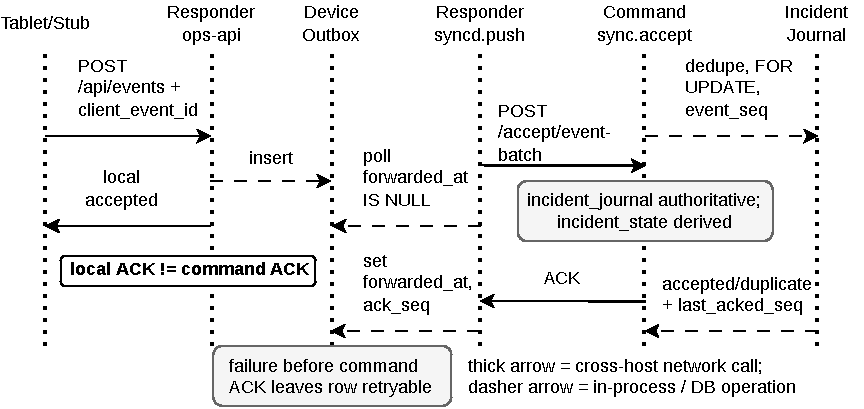
\includegraphics[width=\columnwidth]{figures/fig_outbox_sequence.drawio.pdf}
\caption{Responder outbox protocol is the steady-state field-submission path from tablet to incident journal. The journal assigns the authoritative sequence number, and duplicate delivery is handled by \textit{client\_event\_id}.}
\label{fig:outbox-sequence}
\end{figure}

The M3 contract has three parts:
\begin{enumerate}
  \item Each submission has a globally unique idempotency key, \textit{client\_event\_id}, scoped by the incident and originating client identity.
  \item A responder accepts a submission only after the event is stored in its local outbox.
  \item A responder may mark an outbox item forwarded only after the command edge acknowledges durable incident-journal acceptance or duplicate recognition.
\end{enumerate}

Outbox delivery is at least once and is deduplicated at the command edge; there is no
claim of causal ordering across independent responder outboxes before the command edge
orders them.

\subsection{Fenced Promotion (M4)}
\label{sec:protocol-m4}

M4 moves the command role and provides authority. There is no autonomous failover: an
operator decides that command moves, and M4 keeps the core's journal single-writer
across the move.

\textit{Epochs and the holder check.} The regional core issues each command tenure an
epoch, per incident; the edge taking authority does not choose it. Core issuance gives
promotions on independent vehicles a single order, since each edge owns its database and
an edge-local counter cannot distinguish two edges that both believe they lead. The
epoch is a fencing token in the usual sense~\cite{kleppmann2017ddia}. Every journal
entry carries its epoch, and the core accepts forwarded entries only from the node
recorded as holding the current epoch. Checking the node, not only the number, matters
because a demoted edge that reconnects can read the current epoch from the core. The
check is a protocol boundary, not authentication (\S~\ref{sec:non-claims}).

\textit{Promotion.} The operator first confirms that the old command edge is
unreachable. The candidate then copies the journal prefix held by the core and verifies
that it is contiguous; the core issues the next epoch, and its insert orders concurrent
attempts; only then does the role change. Promotion therefore needs the candidate to
reach the core, but it does not wait for the old command edge.

\textit{The lease.} A cut-off former command edge cannot learn that its epoch is stale,
so it must stop by itself. Write authority is a lease~\cite{gray1989leases} renewed at
the core, on traffic and on an idle heartbeat. A command edge that has not reached the
core for the lease length $L$ stops accepting decisions: on a timer, not on being told.

\begin{figure}[t]
\centering
% Promotion while the command edge is cut off: the case M4 has to handle.
% Hand-drawn TikZ rather than a plot -- the message is the order of events and
% where each entry ends up, which is a layout property, not a data property.
% Colours follow main.tex: accepting path blue (accept), refusal orange (fence).
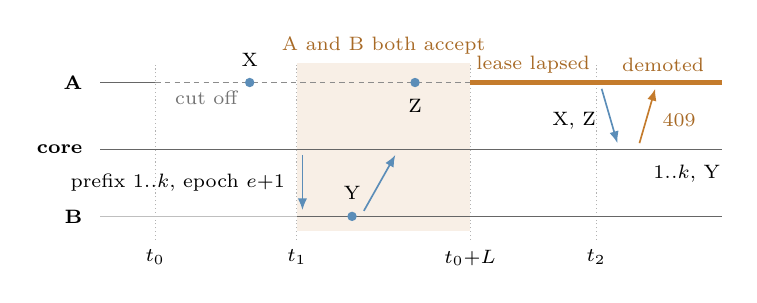
\begin{tikzpicture}[
  x=1cm, y=1cm,
  font=\scriptsize,
  lane/.style={draw=black!60, line width=0.6pt},
  idle/.style={draw=black!25, line width=0.6pt},
  cutlane/.style={draw=black!45, line width=0.6pt, dash pattern=on 2pt off 1.5pt},
  fenced/.style={draw=fence, line width=1.6pt},
  entry/.style={circle, fill=accept, inner sep=1.2pt},
  msg/.style={-{Latex[length=1.5mm,width=1.2mm]}, draw=accept, line width=0.6pt},
  nak/.style={-{Latex[length=1.5mm,width=1.2mm]}, draw=fence, line width=0.6pt},
  tmark/.style={draw=black!30, densely dotted},
]
% Overlap window: after B is promoted and before A's lease lapses.
\fill[fence!12] (3.1,-0.18) rectangle (5.3,1.95);
\node[color=fence!85!black] at (4.2,2.17) {A and B both accept};

% Time marks.
\foreach \x/\t in {1.3/{$t_0$}, 3.1/{$t_1$}, 5.3/{$t_0{+}L$}, 6.9/{$t_2$}} {
  \draw[tmark] (\x,-0.3) -- (\x,1.95);
  \node[anchor=north] at (\x,-0.3) {\t};
}

% Lane labels.
\node[anchor=east, font=\scriptsize\bfseries] at (0.5,1.7) {A};
\node[anchor=east, font=\scriptsize\bfseries] at (0.5,0.85) {core};
\node[anchor=east, font=\scriptsize\bfseries] at (0.5,0.0) {B};

% Lane A: connected, cut off but accepting, lease lapsed, demoted.
\draw[lane]    (0.6,1.7) -- (1.3,1.7);
\draw[cutlane] (1.3,1.7) -- (5.3,1.7);
\draw[fenced]  (5.3,1.7) -- (8.5,1.7);
\node[color=black!55] at (1.95,1.5) {cut off};
\node[entry] (x) at (2.5,1.7) {};
\node[above=0.5pt] at (x.north) {X};
\node[entry] (z) at (4.6,1.7) {};
\node[below=0.5pt] at (z.south) {Z};
\node[color=fence!85!black] at (6.1,1.93) {lease lapsed};
\node[color=fence!85!black] at (7.75,1.93) {demoted};

% Core lane.
\draw[lane] (0.6,0.85) -- (8.5,0.85);
\node[anchor=north] at (8.05,0.78) {$1..k$, Y};

% Lane B: responder until promoted at t1, then command edge.
\draw[idle] (0.6,0.0) -- (3.1,0.0);
\draw[lane] (3.1,0.0) -- (8.5,0.0);
\node[entry] (y) at (3.8,0.0) {};
\node[above=0.5pt] at (y.north) {Y};

% Promotion at t1: B copies the core's prefix and receives epoch e+1.
\draw[msg] (3.17,0.78) -- (3.17,0.08);
\node[anchor=east] at (3.07,0.43) {prefix $1..k$, epoch $e{+}1$};
% B forwards Y.
\draw[msg] (3.95,0.07) -- (4.35,0.78);

% Reconnection at t2: A forwards X, the core refuses, A demotes itself.
\draw[msg] (6.97,1.62) -- (7.17,0.93);
\node[anchor=east] at (7.02,1.22) {X, Z};
\draw[nak] (7.45,0.93) -- (7.65,1.62);
\node[anchor=west, color=fence!85!black] at (7.62,1.22) {409};
\end{tikzpicture}

\caption{Promotion while the command edge A is cut off, with lease length $L$. A is cut
off at $t_0$ and keeps accepting decisions, such as X, that it cannot forward. At $t_1$
an operator promotes B: B copies the core's prefix $1..k$, receives epoch $e{+}1$, and
accepts Y. Until A's lease lapses at $t_0{+}L$, both edges accept (shaded), and A
accepts Z. When A reconnects at $t_2$, the core refuses X and Z with HTTP~409 and A
demotes itself. The core's journal holds $1..k$ and Y; X and Z stay on A.}
\label{fig:promotion-timeline}
\end{figure}

\textit{What M4 guarantees.} In Figure~\ref{fig:promotion-timeline}, B takes authority
at once while A accepts until its lease lapses, so for up to $L$ both edges accept
decisions. The core's journal still never takes entries from two holders, and the
refused edge demotes itself and raises an operator alert. What A accepted but never
forwarded stays on A: decisions from its legitimate tenure (X) as well as from the
overlap (Z). Neither is merged, so the incident record is incomplete until an operator
reviews them.

\textit{Choosing $L$.} The same lease stops a legitimate command edge that has lost only
its backhaul, so $L$ sets \systemname{}'s position in the trade-off of
\S~\ref{sec:tradeoff}. A longer lease keeps decisions flowing through longer outages; a
shorter one narrows the window in which two edges accept. The prototype uses $L=90$\,s
by default. Waiting out the old lease before promotion would close the window, at the
cost of delaying each such promotion by up to $L$ (\S~\ref{sec:alternatives}).

\section{Prototype and Evaluation}
\label{sec:implementation}

\subsection{Prototype and Emulation Setup}
\label{sec:eval-env}
\label{sec:validation}
\label{sec:evaluation}

The artifact repository contains a prototype service path for the core and edge tiers,
plus deployment scaffolding for the target vehicle environment. Services target
Python~3.12 with FastAPI and asyncpg; Docker Compose instantiates the emulated core,
command edge, and responder edges used below, and a separate \textit{baseline/crdt}
stack provides the CRDT-LWW comparison point.

Table~\ref{tab:impl-mapping} records the prototype evidence boundary for each
protocol concept from \S~\ref{sec:architecture}. We use three evidence levels
throughout: \emph{measured} (exercised on
the prototype service path), \emph{model-level} (established by the TLA+/Hypothesis
checks but not the service path), and \emph{deployment-only} (target-deployment
design, not exercised here).

\begin{table}[!htbp]
\centering
\caption{Prototype evidence boundary for each protocol concept.}
\label{tab:impl-mapping}
\scriptsize
\setlength{\tabcolsep}{2pt}
\begin{tabularx}{\columnwidth}{@{}p{0.34\columnwidth}X@{}}
\toprule
\textbf{Concept} & \textbf{Status} \\
\midrule
\multicolumn{2}{@{}l}{\textit{M1--M2: Authority boundary and incident-journal sequencing}} \\
\midrule
Incident journal and \textit{event\_seq} &
Measured on command-edge \textit{syncd} accept. \\
Command-edge accept during responder partition &
Measured on direct command-edge \textit{syncd} accept during responder isolation; command \textit{ops-api} not exercised. \\
\midrule
\multicolumn{2}{@{}l}{\textit{M3: Durable outbox and idempotency}} \\
\midrule
Responder durable outbox &
Measured for responder forwarding. \\
\textit{client\_event\_id} idempotency &
Measured by duplicate replay (\S~\ref{sec:eval-m3}). \\
\midrule
\multicolumn{2}{@{}l}{\textit{M4: Fenced promotion}} \\
\midrule
Promotion and fencing &
Measured across two independent vehicle edges: core-issued per-incident epochs, journal-prefix bootstrap, epoch-holder binding, and lease-based self-fencing (\S~\ref{sec:eval-promotion}). Strict promotion in TLA+; two-edge handoff in Hypothesis. \\
\midrule
\multicolumn{2}{@{}l}{\textit{Supporting infrastructure (not authority-aligned)}} \\
\midrule
Core bootstrap, backhaul, and journal forwarding &
Synthetic bootstrap/backfill in Docker; forwarding measured for WAN recovery. \\
Vehicle edge roles and tablet client &
Command and responder edges in Compose; Python stub in evaluation, Android scaffold only. \\
Netem evaluation, transit and security controls &
Measured under two link profiles (\S~\ref{sec:eval-m3}); physical mesh and security overhead are deployment design only, out of scope. \\
\bottomrule
\end{tabularx}
\end{table}

Security controls (VPN overlay, mTLS termination, certificate-derived identity)
are deployment design, not measured here; the emulation uses plain HTTP on a
Docker bridge with synthetic device and user identifiers.

We evaluate the prototype on a single-host emulation, organized by the four
mechanisms of \S~\ref{sec:architecture} (M1--M2, M3, and M4).
Three
further experiments delimit what \systemname{} does not promise rather than
evaluate a mechanism--a Raft consensus baseline (\S~\ref{sec:eval-raft}), a
CRDT-LWW semantic falsification (\S~\ref{sec:eval-crdt}), and command-to-core
WAN backhaul recovery (\S~\ref{sec:eval-wan}). Finally,
\S~\ref{sec:eval-network} varies the two axes the mechanism cells hold fixed:
connectivity over time, and the number of responder edges.

The propagation, recovery, and
throughput cells use a single responder path, so reported latencies are per-path,
not aggregate. Each cell repeats $n=30$ unless noted, with median and p95
reported. Partitions cut only the targeted path with \textit{tc}, so each cell
isolates one effect.
Impairment uses two \textit{tc-netem} profiles informed by published mesh
measurements~\cite{zimbelman2022mesh,kumbhar2015legacy}.
Table~\ref{tab:evaluation} collects the primary service-path numbers.

\begin{table}[t]
\centering
\caption{Service-path measurements for responder propagation, WAN recovery, command serialization, and responder isolation.}
\label{tab:evaluation}
\scriptsize
\setlength{\tabcolsep}{3pt}
\begin{tabularx}{\columnwidth}{@{}p{0.34\columnwidth}p{0.25\columnwidth}X@{}}
\toprule
\textbf{Path / cell} & \textbf{Result} & \textbf{Interpretation} \\
\midrule
% Auto-generated by scripts/generate_tables.py.
% Do not edit; re-run the script after evaluation JSONL changes.
\textit{Responder-to-command propagation} & & \\
  \hspace{2mm}queue depth = 1 ($n=30$) & median 710.1\,ms; p95 832.1\,ms & outbox-to-command journal path \\
  \hspace{2mm}queue depth = 10 ($n=30$) & median 639.4\,ms; p95 719.5\,ms & outbox-to-command journal path \\
  \hspace{2mm}queue depth = 100 ($n=30$) & median 931.5\,ms; p95 1045.5\,ms & outbox-to-command journal path \\
\addlinespace
\textit{Command-to-core WAN recovery} & & \\
  \hspace{2mm}partition = 1\,s ($n=30$) & median 0.75\,s; p95 0.92\,s & support-path backhaul, not command authority \\
  \hspace{2mm}partition = 10\,s ($n=30$) & median 0.91\,s; p95 1.04\,s & support-path backhaul, not command authority \\
  \hspace{2mm}partition = 60\,s ($n=30$) & median 0.23\,s; p95 1.05\,s & support-path backhaul, not command authority \\
\addlinespace
\textit{Command journal serialization} & & \\
  \hspace{2mm}direct \texttt{/accept} ($n=29$) & median 356.3 events/s; p95 491.7 & sequencer: command accept + journal write only \\
  \hspace{2mm}end-to-end via outbox ($n=29$) & median 159.4 events/s; p95 163.9 & full responder outbox $\rightarrow$ push-batch $\rightarrow$ command path \\
\addlinespace
\textit{Command commit during responder isolation} & & \\
  \hspace{2mm}direct command accept path ($n=20$) & 20/20 commits; seq. 1--20; 0 duplicate seqs. & direct \texttt{/accept/event-batch} path; median/p95 latency 5.76/7.32\,ms \\
\bottomrule

\end{tabularx}
\end{table}

\subsection{Authority boundary and journal sequencing (M1--M2)}
\label{sec:eval-independence}
\label{sec:eval-m1}
\label{sec:eval-m2}

M1--M2 serve R3, and R1 for command-side writes.

With one responder isolated for ten seconds, direct single-event POSTs to
\textit{/accept/event-batch} all commit, assigning consecutive non-duplicate
\textit{event\_seq} values at single-digit millisecond latency
(Table~\ref{tab:evaluation}). Stale or absent \textit{X-Command-Epoch} values are
rejected before journal work. Responder reachability is therefore not in the commit
path.

Saturation throughput at the linearization point (Table~\ref{tab:evaluation})
reflects a single-writer serializer. Even a generous 10 authority-bearing events
per minute is 0.17 events/s, so the measured 356.3 events/s exceeds plausible
incident demand by three orders of magnitude.

\subsection{Durable outbox and idempotent submission (M3)}
\label{sec:eval-m3}

M3 (the durable responder outbox with \textit{client\_event\_id} idempotency)
serves R1 and R2.

Median propagation stays sub-second across queue depths 1--100; the p95 at
depth 100 marginally exceeds 1~s (1045.5~ms, Table~\ref{tab:evaluation}).

Replaying 50 unique \textit{client\_event\_id} values five times each leaves exactly 50
journal rows across $n=30$ runs: forwarding is at-least-once and deduplicated at the
journal, so submission is effectively exactly-once at the linearization point. Across
process restart, 50 outbox submissions survive a responder-Postgres power cycle, then
forward with no duplicates and consecutive \textit{event\_seq}, reaching journal
consistency about 2.6\,s after recovery---the runtime witness for R2.

\subsection{Fenced promotion (M4)}
\label{sec:eval-promotion}
\label{sec:eval-m4}

M4 (fenced promotion with stale-epoch rejection) serves R3 under command transfer and
exercises C2: promotion preserves single authority across an epoch change and rejects
stale-epoch traffic, on the service path, before any incident-journal work.

Protocol cost is single-digit milliseconds across all three phases of a transition
(Figure~\ref{fig:promotion-cost}). Commit phases~$A$ and~$C$ have medians
\promotionMedianA{} and \promotionMedianC{}; the phase~B stale-rejection path is
$2.5\times$ cheaper by construction, since the fence rejects stale traffic before the
journal write. Operator confirmation sits in the critical path by design and dominates
wall-clock; the protocol contribution is orders of magnitude smaller, an operator cost
rather than a network cost.

\begin{figure}[t]
\centering
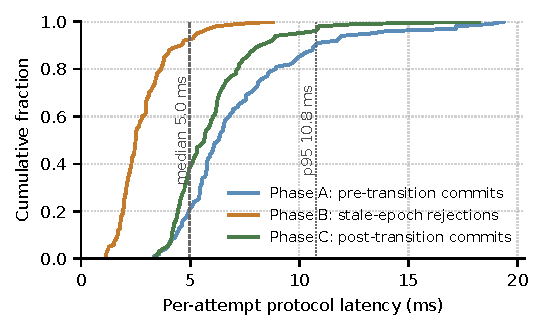
\includegraphics[width=0.85\columnwidth]{figures/fig_promotion_cost.pdf}
\caption{Fenced-promotion protocol cost by phase. Phase~A is pre-transition
commits at epoch~$e$, phase~B is stale-epoch rejections at the journal boundary,
phase~C is post-transition commits at epoch~$e+1$. $n=\promotionN$ events
($\promotionNPerPhase$ per phase). Vertical markers are pooled across phases:
median \promotionMedianCombined{}, p95 \promotionPNinetyFiveCombined{}. The
cost shown is the protocol path only; the operator-confirm step is excluded by
design.}
\label{fig:promotion-cost}
\end{figure}

In five live service-path runs, phase~$A$ commits 20/20 events at epoch~1, phase~$B$
returns 20/20 HTTP~409 rejections for the stale epoch and adds zero
incident-journal rows, and phase~$C$ commits 20/20 events at epoch~2. The incident
journal holds 200 rows total, split 100/100 between epochs, with no
\textit{event\_seq} value appearing under both.

\subsubsection{Two-edge fenced promotion}
\label{sec:eval-two-edge}

The results above hold at one acceptor. We additionally exercise promotion across two
independent vehicle edges, each with its own database, with the incumbent partitioned
from the network. The candidate bootstraps the journal prefix from core, verifies it is
contiguous, obtains the next epoch, and only then takes the role; responders are
repointed at the new command.

Two outcomes matter for R3, and both are measured rather than asserted. First, when the
superseded edge reconnects and forwards the writes it buffered while isolated, core
refuses them because another node holds the epoch; the edge demotes itself, and its own
accept path then refuses authority-bearing writes. Its buffered rows are retained for
reconciliation, and the authoritative journal is unchanged throughout---the fork
is contained at the
journal boundary and never admitted. Second, when the \emph{current} holder
loses only its backhaul, it accepts writes while its lease is valid and refuses them
once the lease lapses, recovering when the link returns. It is never informed that
anything happened; it stops on a timeout it cannot renew, which is the honest form of
the guarantee and the reason the availability cost falls where it does.

We do not report a fencing latency here. The transition is dominated by the
lease window, an operator-chosen parameter rather than a property of the
protocol, and the operator confirmation step already dominates wall-clock
(\S~\ref{sec:eval-promotion}).

Verification and falsification costs are strongly asymmetric. The strict variant passes
all six safety invariants over 38.56\,M distinct states in 13.0\,min, whereas each weak
variant is refuted almost immediately: \textit{SingleAuthority} in 185 states (0.85\,s),
\textit{EpochAuthorityCoupling} in 144 (0.77\,s), and \textit{NoForkedJournal} in 1.0\,k
(0.83\,s). Establishing the property is expensive; refuting the weakened rule is not.

\subsection{Scope Boundaries}

\subsubsection{Raft leadership follows the reachable quorum}
\label{sec:eval-raft}

This tests the R3-relevant mismatch between consensus leadership and operational
command authority. The baseline is the three-voter \textit{hashicorp/raft} cluster in
\textit{baseline-raft/}. Each run hard-cuts the current leader $L_0$ from the other
two voters; the reachable majority elects $L_1$ and accepts writes there
(Table~\ref{tab:raft-comparison}). This is correct Raft
behavior---authority moves to a node that can form a quorum~\cite{ongaro2014raft}---and
it is exactly the mechanism mismatch for R3: Raft has no input by which an operator
can pin the writer to an externally designated command edge.


\begin{table*}[t]
\centering
\caption{Raft consensus baseline. Authority follows the reachable quorum, not an
operator-designated command edge.}
\label{tab:raft-comparison}
\scriptsize
\setlength{\tabcolsep}{3pt}
\begin{tabularx}{\textwidth}{@{}p{0.16\textwidth}p{0.39\textwidth}X@{}}
\toprule
\textbf{Scenario} & \textbf{Measured result} & \textbf{Interpretation} \\
\midrule
% Auto-generated by scripts/generate_raft_table.py.
% Do not edit; re-run the script after Raft evaluation JSONL changes.
Event sequencing sanity & leader batch accepted 1 event, deduplicated 1, last seq. 1; journal count 1 & Confirms the Raft FSM assigns \textit{event\_seq} and enforces \textit{client\_event\_id} idempotency. \\
Leader-minority partition & 12/12 runs elected $L_1 \ne L_0$; 12/12 committed 5 writes at $L_1$; new-leader median 3.08\,s, p95 4.43\,s & $L_0$ writes while isolated, during the election: stall then apply timeout 12/12. Once it has stepped down it instead refuses up front, 12/12, at 0.4\,ms against 269.9\,ms in-window. Authority follows the reachable quorum, not an external command designation. \\
\bottomrule

\end{tabularx}
\end{table*}

\subsubsection{CRDT semantics fail for authority-bearing data}
\label{sec:eval-crdt}

This tests C1: mergeable-by-default replication cannot encode authority for
non-commutative incident decisions. It is a semantic falsification, not a speed
comparison.

The CRDT-LWW baseline is four FastAPI replicas using Hanssen's operation-based
Last-Writer-Wins Element Set~\cite{hanssen2025emergency}. It preserves local
acceptance but loses authority-bearing conflicts: concurrent status updates
converge to the latest timestamp, and a later update resurrects a deleted
element. LWW discards the losing status from materialized state, whereas AAL
preserves both writes in an attributed total order. Ordering and attribution are
R3's service-path scope; semantic rejection is an additional guard disclosed in
\S~\ref{sec:non-claims}.

The baseline is deliberately lightweight and in-memory, converging only through
harness-triggered \textit{full\_sync()}: the test needs the merge rule exercised on
concurrent authority-bearing writes, not storage parity. The asymmetry favors
CRDT where it already performs better, which is the
correct bias for a falsification: if mergeable-by-default semantics cannot encode
authority even under favorable conditions, the semantic argument holds regardless
of infrastructure differences.
Table~\ref{tab:crdt-comparison} keeps measured AAL behavior, model-level AAL
safety, and measured CRDT-LWW semantics separate.

\begin{table*}[t]
\centering
\caption{Semantic comparison with a Hanssen-style CRDT-LWW baseline. The concurrent-edit and delete/update rows use \emph{constructed} conflicts, so their 30/30 outcomes are deterministic by design, not sampled.}
\label{tab:crdt-comparison}
\scriptsize
\setlength{\tabcolsep}{3pt}
\begin{tabularx}{\textwidth}{@{}p{0.16\textwidth}p{0.24\textwidth}p{0.25\textwidth}X@{}}
\toprule
\textbf{Scenario} & \textbf{AAL result} & \textbf{CRDT-LWW result} & \textbf{Interpretation} \\
\midrule
% Auto-generated by scripts/generate_tables.py from eval_crdt_baseline.anon.jsonl.
Field-edit propagation & Attributed order preserved; unimpaired service-path medians in Table~\ref{tab:evaluation} & Impaired: qd=10 stressed/degraded 814.1\,ms/2.54\,s; qd=100 degraded 3.97\,s & Measured under different link conditions, so not a latency comparison; both preserve durable propagation, and CRDT anti-entropy is not an authority boundary. \\
Concurrent status edit & Measured prototype path sequences unique events; semantic rejection is model-level/not implemented in that path & 30/30 LWW runs converge; winner counts contained: 30; median 12.8\,ms & LWW accepts both writes and materializes only the latest value; losing op is only recoverable from the op log. \\
Delete/update race & Measured prototype path has no delete/update semantic guard; limitation disclosed & 30/30 runs resurrect the element; median convergence 12.7\,ms & Matches Hanssen's stated LWW delete-semantics caveat. \\
No-partition throughput & Prototype command-journal commit rate median 356.3 events/s (single writer) & CRDT aggregate local accept rate across three writers median 349.2 events/s & Different units; reports write-availability trade-off, not direct speedup. \\
Post-quiescence convergence (60\,s outage, $n=10$) & Prototype command-to-core support-path recovery median 227.0\,ms after a real \textit{tc} WAN cut ($n=30$) & CRDT all-replica convergence median 45.4\,ms after anti-entropy resumes (no link impairment during the wait) & Comparable in outage duration, not transport mechanism; \systemname{} keeps command-local ordering, CRDT converges once anti-entropy is exchanged. \\
\bottomrule

\end{tabularx}
\end{table*}

\subsubsection{Backhaul recovers within about a second of WAN heal}
\label{sec:eval-wan}

This measures command-to-core forwarding after a WAN heal, with a narrowly
targeted \textit{tc} cut of the command-to-core path only, so the measurement
isolates backhaul flush time (Table~\ref{tab:evaluation}). Recovery is bounded
by the forward poll loop and backlog, not outage length, so
non-monotonic medians across 1, 10, and 60~s outages are expected poll-phase effects.

\subsection{Time-varying connectivity and fleet size}
\label{sec:eval-network}

The measurements above hold connectivity fixed for the duration of a cell and
use a single responder. Neither matches a rescue deployment: vehicle
connectivity alternates between regimes, and incidents involve several
responders at once. This subsection varies each axis in turn.

\subsubsection{Regime transitions, not steady state}
\label{sec:eval-schedule}

A single continuous submission stream runs while the responder-to-command path
walks a schedule of regimes---clear, mesh-stressed, mesh-degraded, isolated,
clear---and every event is attributed to the regime in force when it was
submitted. Impairment is destination-filtered, so only the peer path is
affected and each edge keeps full-speed access to its own database. Ten runs of
the schedule submit 540 events in total.

The result is the durable-outbox property observed \emph{across} a transition
rather than inferred from steady state (Table~\ref{tab:netem-schedule}). Under
every degraded-but-connected regime, delivery within the phase is complete.
Under isolation it is zero: no event reaches the authoritative journal while the
path is down, which is the honest statement of what a single-writer boundary
costs. No event is lost. All 540 reach the journal, all ten runs drain fully,
and the outbox backlog peaks at 13 events before collapsing once the link
returns. Recovery---measured from the instant connectivity is restored until
every event pending at that instant is journal-visible---is sub-second across
all ten runs, with a measurement resolution of about 0.4~s set by the polling
interval and query cost. It is bounded by the forwarder's poll cycle and the
backlog depth, not by how long the outage lasted.

\begin{table}[t]
\centering
\caption{Delivery across a connectivity-regime schedule, $n=10$ runs, 540
events. \emph{Within phase} counts events journaled before that phase ended;
\emph{eventually} counts them after the link returns. The gap between the two
columns in the isolated row is the durable outbox doing its job.}
\label{tab:netem-schedule}
\footnotesize
\setlength{\tabcolsep}{5pt}
\begin{tabular}{@{}lrr@{}}
\toprule
\textbf{Regime} & \textbf{Delivered within phase} & \textbf{Delivered eventually} \\
\midrule
% Auto-generated by scripts/generate_network_tables.py.
% Do not edit; re-run the script after evaluation JSONL changes.
Clear & 1.00 & 1.00 \\
Mesh, stressed & 1.00 & 1.00 \\
Mesh, degraded & 1.00 & 1.00 \\
Isolated & 0.00 & 1.00 \\
Clear (restored) & 1.00 & 1.00 \\
\bottomrule

\end{tabular}
\end{table}

\subsubsection{Fleet size}
\label{sec:eval-fleet}

The second axis is the number of responder edges submitting concurrently.
\S~\ref{sec:eval-m1} argues that a single-writer serializer is adequate because
its saturation rate exceeds plausible incident demand; that argument is only as
good as its behaviour when responders multiply. Fleet sizes of 1, 3, 5 and 10
independent responder edges---each with its own database and outbox---submit
simultaneously, five runs each, 20 events per responder
(Table~\ref{tab:fleet-scaling}).

Delivery is complete at every size: 1900 of 1900 events across the sweep. Journal
throughput rises from 19.5 to 182.5 events/s, a factor of 9.4 for a tenfold
increase in offered load, while propagation latency does not degrade---the p95
at ten edges is below the value at five. The single-writer linearization point
therefore absorbs a ten-edge fleet without becoming the bottleneck, which is the
measured form of the claim \S~\ref{sec:eval-m1} makes.

Two limits are worth stating. The throughput figures are not comparable to the
saturation rate in Table~\ref{tab:evaluation}: a 200-event batch is dominated by
fixed per-event latency, not by serializer capacity, so these numbers are a
lower bound on both. And ten edges is where this single host runs out of memory,
not where \systemname{} runs out of headroom---73 containers share one kernel,
one disk and one bridge. What the sweep establishes is the shape of the curve,
not an absolute ceiling.

\begin{table}[t]
\centering
\caption{Concurrent responder edges against the same command edge, five runs per
size, 20 events per responder. Percentiles are arrival-curve percentiles: the
time by which the journal held that share of the batch.}
\label{tab:fleet-scaling}
\footnotesize
\setlength{\tabcolsep}{4pt}
\begin{tabular}{@{}rrrrr@{}}
\toprule
\textbf{Edges} & \textbf{p50} & \textbf{p95} & \textbf{Events/s} & \textbf{Delivered} \\
\midrule
% Auto-generated by scripts/generate_network_tables.py.
% Do not edit; re-run the script after evaluation JSONL changes.
1 & 1.02\,s & 1.02\,s & 19.5 & 1.00 \\
3 & 606.7\,ms & 963.9\,ms & 62.2 & 1.00 \\
5 & 643.7\,ms & 1.35\,s & 74.2 & 1.00 \\
10 & 728.4\,ms & 1.10\,s & 182.5 & 1.00 \\
\bottomrule

\end{tabular}
\end{table}

Neither experiment is a mobility model. No vehicle positions, path loss or RAN
topology are simulated; the regime durations and impairment parameters are
literature-informed and the transitions are synthetic, which is what makes them
reproducible.

Every cell leaves the authority boundary where \S~\ref{sec:architecture} places
it: no forked journal, no submission lost, no write admitted from a node that
does not hold the epoch. \S~\ref{sec:non-claims} details the non-claims.

\section{Discussion}
\label{sec:discussion}

\subsection{Designated and Plural Authority}
\label{sec:thesis}

This paper covers one class of decision: a command decision, which gets its legitimacy
from one designated person's role, takes effect when it is issued, and is settled by
authority, never by merge, when it conflicts with another. It binds when it is admitted to
the authoritative journal under a valid grant. Decisions whose authority is shared or
contested belong to the opposite pole, where legitimacy comes from agreement among
several parties and a decision binds only at reconciliation; there, merge or consensus is
the right tool. The class of decision, not the state of the network, chooses between the
two. Our earlier design let reachability choose the commander; the model of
\S~\ref{sec:system-model} removes that.

The boundary is also where this paper stops. \systemname{} defines residual decisions,
attributes them and labels them; it does not resolve them. Deciding what happens to an
order issued under a superseded grant---confirm it, reverse it, or let the new commander
rule on it---is a reconciliation that acts on command decisions, and we leave it to
future work that composes the two poles.

\subsection{Security Assumptions}

The target deployment assumes an organizational CA with enrolled devices and users, and
the model assumes credentials are not stolen. Revocation of a stolen tablet or vehicle
node is eventual under total disconnection, and a captured command edge can poison the
journal for as long as its holder's grant is valid; a quorum-inferred design fails
differently, not better, by moving authority away from the designated commander. The
design relies on signed grants, fencing and audit, not on Byzantine tolerance.

\subsection{Evaluation Boundaries and Non-claims}
\label{sec:non-claims}
\label{sec:alternatives}

The paper does not claim that \systemname{} solves succession under partition: the
trade-off rules that out, and the prototype realizes only S1. The claims about S0 and
S2--S5 in Table~\ref{tab:policies} are hypotheses until the comparison of
\S~\ref{sec:eval-policies} has been run.

Both formal models cover coordinated handover only. The TLA+ model has one shared
journal and promotes only when the old command edge is reachable; the Hypothesis handoff
model promotes only after the old command edge has forwarded its whole journal; neither
has a lease. Model checking therefore establishes the six invariants for that case. The
cut-off case of Figure~\ref{fig:promotion-timeline} has a runtime witness only, and in it
\textit{DurabilityAcrossPromotion} does not hold for entries the old command edge never
forwarded.

The prototype's gaps against the model are listed in \S~\ref{sec:model-gap}. In
addition, \systemname{} records decisions but does not deliver them to responder edges;
any delivery acknowledgement must not block, since a two- or three-phase commit would
stall every decision while a team is out of coverage (R1). Semantic rejection of
conflicting values is not implemented.

The emulation isolates the authority and replication mechanisms from deployment
variables: physical mesh transport, security overlay cost, and Android client
integration. It does not claim physical Rajant mesh behavior, measured WireGuard or mTLS
overhead, or end-to-end Android validation, and the workload is single-incident and
limited-scale. The connectivity schedule is not a mobility model: no vehicle positions,
path loss, or RAN topology are simulated. Command-side writes are exercised through
\textit{syncd}'s accept path rather than the command \textit{ops-api}, and core bootstrap
and backfill are synthetic rather than measured.

\section{Conclusion}

Command at an incident belongs to a person, and the organization, not the network,
decides who that person is. We separated a person's right to command from a node's right
to write: authority comes from signed grants and a succession rule fixed in advance,
nodes exercise it, a decision binds when it is admitted under a valid grant, and
decisions made under a superseded grant are kept as labelled residuals. While the
commander is cut off, no design can keep the commander recording, move command without
them, and keep one disconnected edge accepting, all at once. Succession is therefore a
choice of policy, and we laid out six policies by what each gives up. The \systemname{}
prototype realizes one of them, immediate promotion through the core with a lease, and we
reported both what it guarantees and where it falls short of the model. Raft moves
authority to the reachable quorum and a last-writer-wins CRDT lets the merge decide;
neither can carry the organization's decision.

\pending{Next: check succession practice with the rescue service, extend the prototype
with persons, grants and policies S0--S4, run the policy comparison across partition cases
P-A to P-C on a multi-host testbed, and model-check each policy with the lease in TLA+.}


\bibliographystyle{IEEEtran}
\bibliography{refs}

\end{document}
